\documentclass[12pt]{report}
\usepackage[utf8]{inputenc}
\usepackage{xcolor}
\usepackage[margin=1in]{geometry}
\usepackage{soul} 
\usepackage{apacite}
\usepackage{graphicx}
\usepackage{xurl}

\usepackage{fancyhdr}
\pagestyle{fancy}

\lhead{Research Project}
\rhead{Draft Chapter 1}
\cfoot{\thepage}
\renewcommand{\headrulewidth}{0.4pt}
\renewcommand{\footrulewidth}{0.4pt}

\title{Alternate Review Systems:\\ Quantifying Enjoyability in Table-top Games}
\author{Jai Bakshi \\ 21060322069}
\date{September 2024}

\begin{document}
	\maketitle
	\chapter{The Dynamics of Snakes and Ladders}
	This chapter will delve into the mechanics of the classic game Snakes and Ladders, aiming to quantify the impact of various game parameters on the overall game dynamics. This is done by simulating numerous games while systematically varying parameters such as the lengths of snakes and ladders and the number of snakes and ladders on the board. To simplify the analysis, the model reduces the game to its essential elements, allowing us to systematically examine how changes in these parameters affect the distribution of game duration - specifically, the number of moves needed to reach the end state.
	\section{Setting up the board}
	In our pilot study, the game board is modelled as a 100-square grid, akin to the classic Snakes and Ladders game. However, to facilitate a systematic investigation of the game dynamics, we introduce certain controllable parameters:
		
		\begin{enumerate}
			\item Number of Snakes ($N_{s}$): The total number of snakes present on the board.
			\item Number of Ladders ($N_{l}$): The total number of ladders on the board.
			\item Length of Snakes ($L^{i}_{s}$): This parameter determines the length of the $i^{th}$ snake on the board for $i=1,2,... N_{s}$. It dictates how far down a player moves when landing on a snake's head.
			\item Length of Ladders ($L^{i}_{l}$): This parameter determines the length of $i^{th}$ ladder on the board for $i=1,2,... N_{l}$. It dictates how far up a player climbs when encountering a ladder's base.
		\end{enumerate}

	To ensure that the configuration of the board remains valid and doesn't present any conflicts such as - positioning snakes or ladders at invalid tiles where they might exceed or precede boundaries of the board, certain constraints are implemented:

	\begin{enumerate}
		\item Ladder Constraint: Ladders cannot begin within the $L^{N_{L}}_{l}$ squares of the board to prevent them from extending beyond the game's end.
		\item Snake Constraint: Snakes cannot begin within the first $L^{1}_{s}$ squares to avoid their tails going below the starting position.
		\item Overlap Constraint: The endpoints of snakes and ladders cannot coincide. If such an overlap occurs, either the snake or the ladder is randomly re-positioned to maintain the game's integrity.
	\end{enumerate}
	
	The board generation process involves randomly selecting starting positions for snakes and ladders within the permissible ranges, followed by a validation step to resolve any overlaps. This iterative process continues until a valid board configuration is achieved. The number of iterations required to generate a valid board is recorded and can be analysed to understand the complexity of board creation under different parameter settings.
	
	This structured approach to board generation allows us to systematically vary the parameters (number of snakes, number of ladders, snake length, ladder length) and study their individual and combined effects on the game dynamics. By analysing the resulting distributions of game durations, we aim to uncover trends and patterns that reveal the interplay of these factors in shaping the player's experience.
	
	\section{Presenting Findings}
	The game of Snakes and Ladders is inherently probabilistic in nature, with the outcome largely being determined by the interplay between board design and randomness in dice rolls. The board design consists of a number of Snakes and Ladders with varying lengths that either move the player down or bring them closer to the goal. Snakes and ladders introduce variability into game dynamics by contracting or extending player movement. This section of the research project focuses on how the number of snakes ($N_{s}$) and ladders ($N_{L}$) affects the average game time. Using simulated data, the project explores the relationship between different configurations of snakes and ladders, keeping their lengths constant while varying their quantities. The game has been simulated 1000 times with 10 distinct board configurations while varying the parameters independently of each other. The analysis is based on three distinct visualisations: box plots, trend lines, and a heatmap, which offer insights into distribution, trends, and overall patterns, respectively.
	
	\subsection{Distribution of Average Game Times}
		\begin{figure}[h]
			\centering
			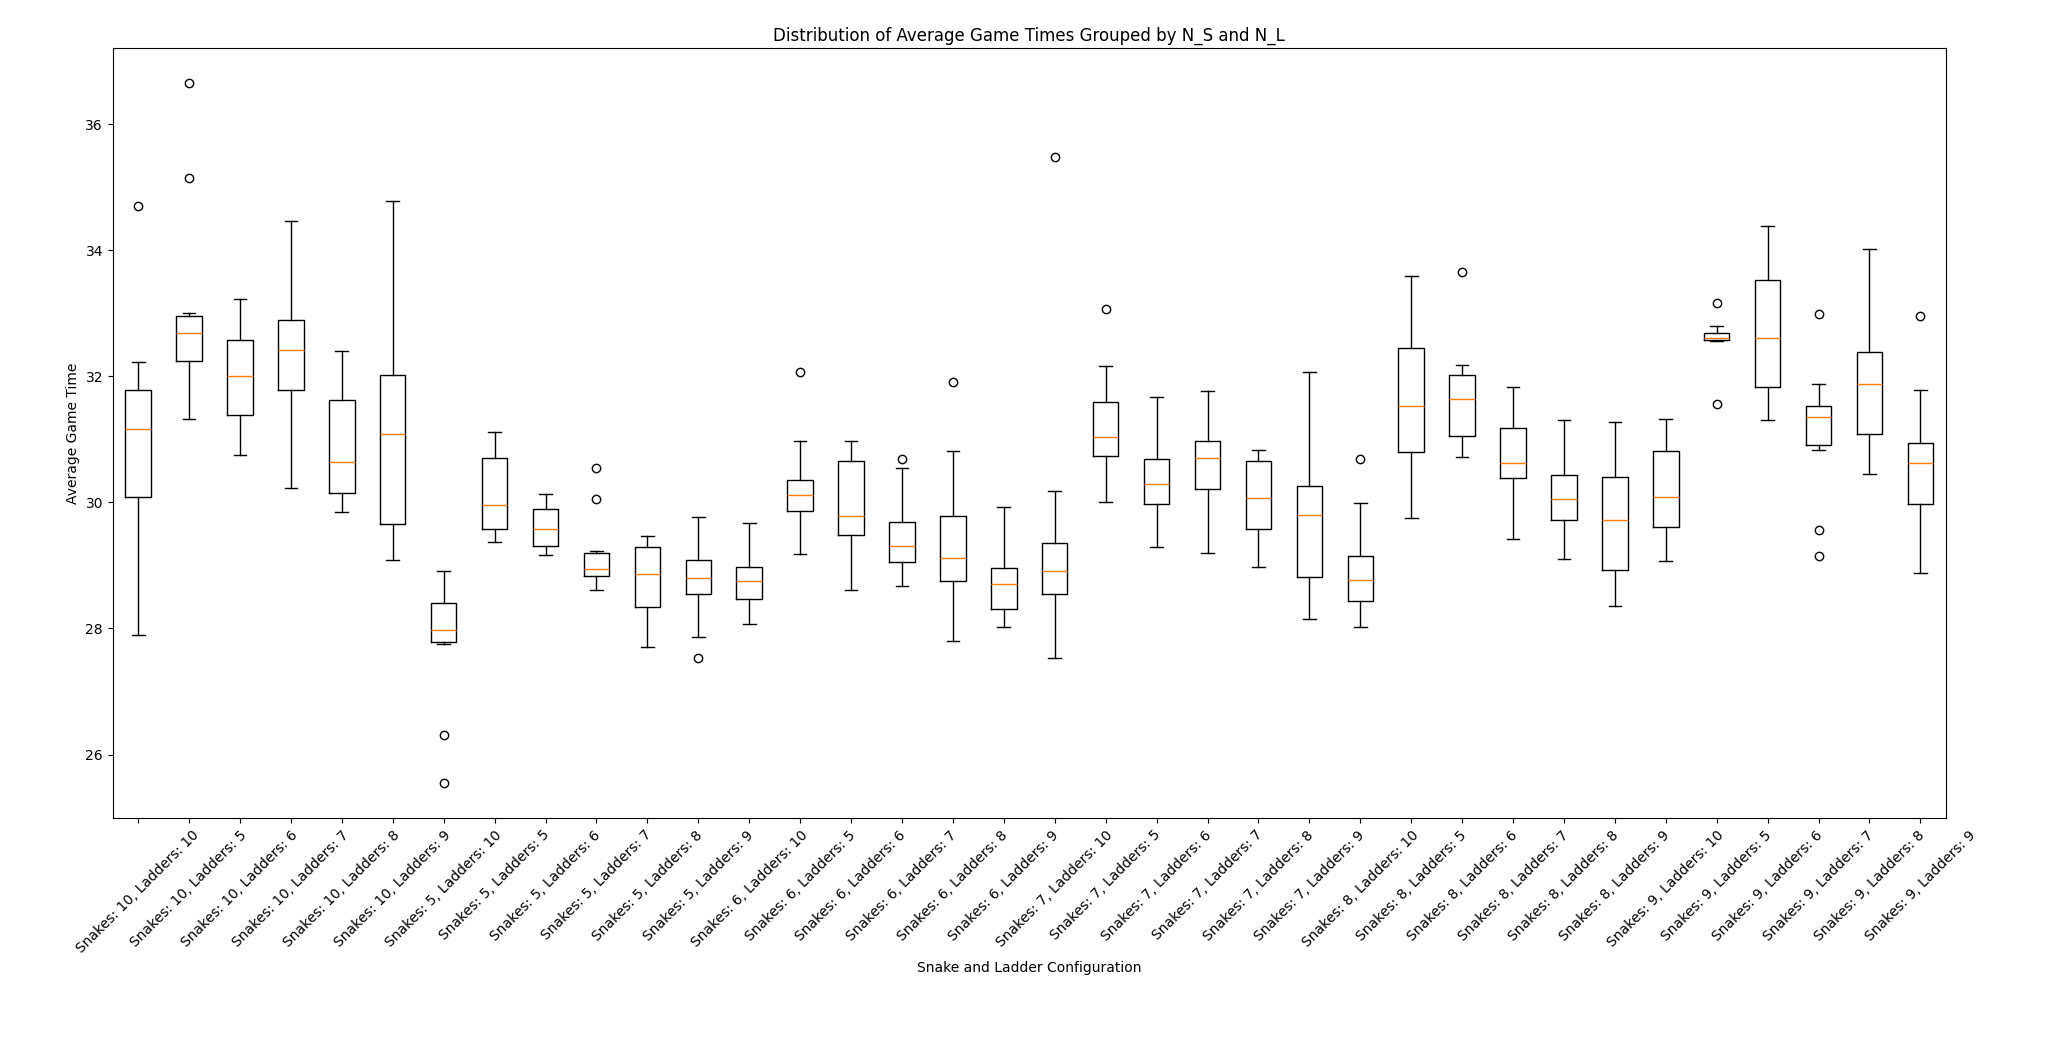
\includegraphics[width=0.8\textwidth]{BoxPlots}
			\caption{Distribution of Average Game Times Grouped by $N_{S}$ and $N_{L}$}
			\label{fig:boxplots}
		\end{figure}
	
	The box plot (fig 1.1) shows the distribution of average game times across various combinations of $N_{s}$ and $N_{L}$. The game configurations that show an extreme difference in the number of snakes and ladders (e.g., $N_{s} = 10$ and $N_{L} = 5$) show the highest variability in average game time. This can be observed through the wider interquartile ranges and more frequent outliers. A key feature is that configurations with fewer ladders tend to have longer game times. For instance, configurations with 10 snakes and 5 ladders frequently have average game times above 33, with a few extreme outliers nearing 37. The average game time tends to decrease as the number of ladders increases. This is intuitive, as ladders facilitate faster movement towards the goal state, reducing the number of turns required to reach the end of the game. For example, configurations with 10 snakes and 9 or 10 ladders have noticeably lower average game times than those with only 5 ladders. The whiskers for these configurations often do not extend beyond 30, suggesting a tighter and more consistent game time with fewer outliers. The plot concludes that outliers are frequent in configurations with more snakes and fewer ladders. This indicates that while these setups generally lead to longer game times, there are instances where luck allows a faster completion. These outliers could represent cases where a player avoided all major snakes, resulting in an unusually short game.
	
	\subsection{Trend in Average Game Times for Different Configurations}
	\begin{figure}[h]
		\centering
		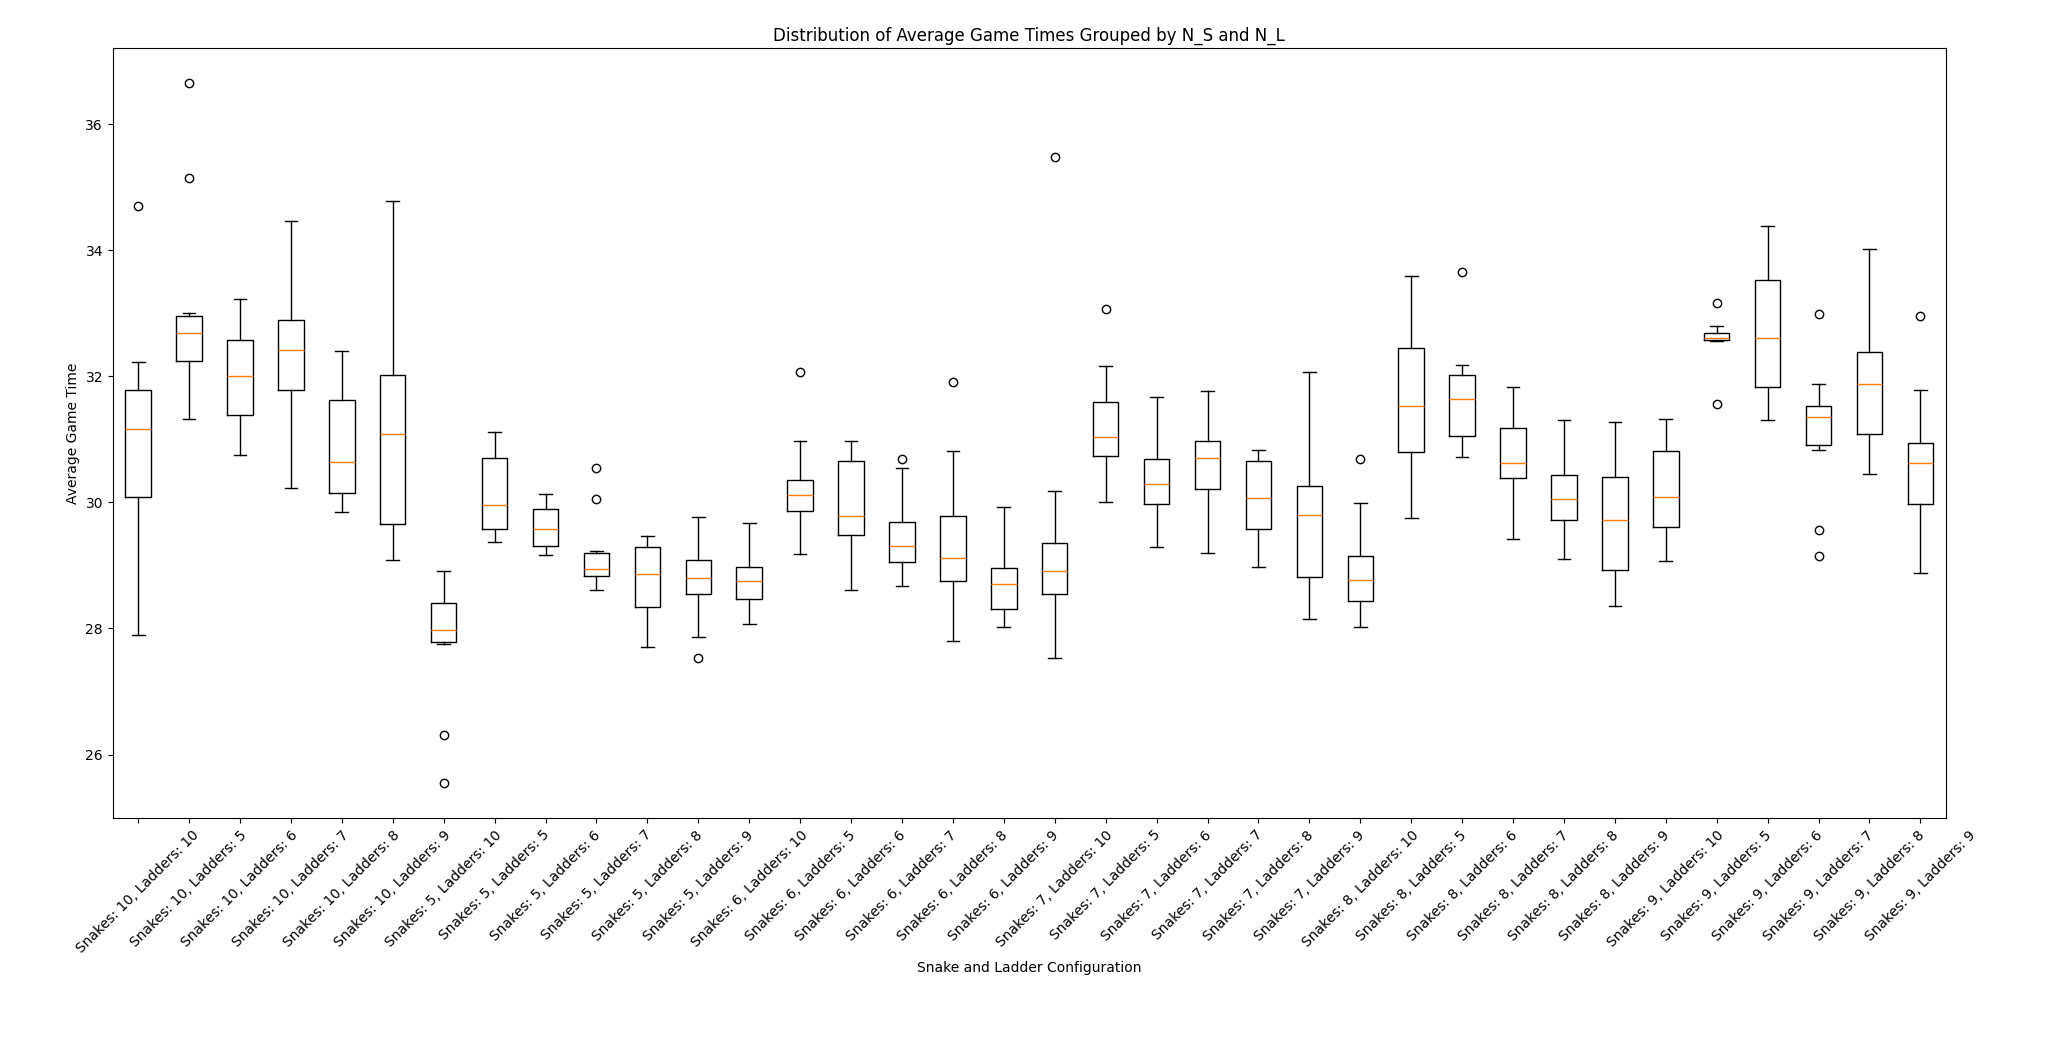
\includegraphics[width=0.8\linewidth]{BoxPlots}
		\caption{Trend in Average Game Times for Different Configurations}
		\label{fig:boxplots}
	\end{figure}
	The line graph (fig 1.2) helps to track trends in average game times across different boards for each configuration of snakes and ladders. This visually compares game performance for each combination as the board layout also changes for each configuration of the parameters. One of the most apparent observations from the trend analysis is that there is a lack of a clear dominant configuration. Although certain combinations appear to result in consistently higher or lower game times, the lines frequently cross each other, indicating that no single combination guarantees the fastest or slowest game across all boards. The line chart shows that the configurations with fewer snakes ($N_{s} = 5, 6$) tend to produce more stable game times, regardless of the number of ladders. These configurations generally have fewer extreme spikes and dips in average game time, as indicated by smoother lines on the graph, i.e. due to the reduction in the risk profile of the board layout, the player’s game time becomes more consistent from run to run. For configurations with higher snake counts ($N_{s} >= 9$), there are noticeable spikes in average game time for certain boards. These spikes suggest that the placement of snakes on specific boards creates significant delays, likely due to frequent encounters with snakes that force players back to multiple spaces. The impact of ladders in these cases is reduced, as the advantage gained from a ladder can be undone by a snake in later turns. Configurations with 9 or 10 ladders generally exhibit less fluctuation across boards. While they may not always have the shortest game times, they provide more consistent results, reducing extreme outliers and spikes. This measure also counters the effect of high counts of snakes, generally stabilising the game mechanics.
	
	\subsection{Interaction Between the Number of Snakes and Ladders}
\begin{figure}[h]
	\centering
	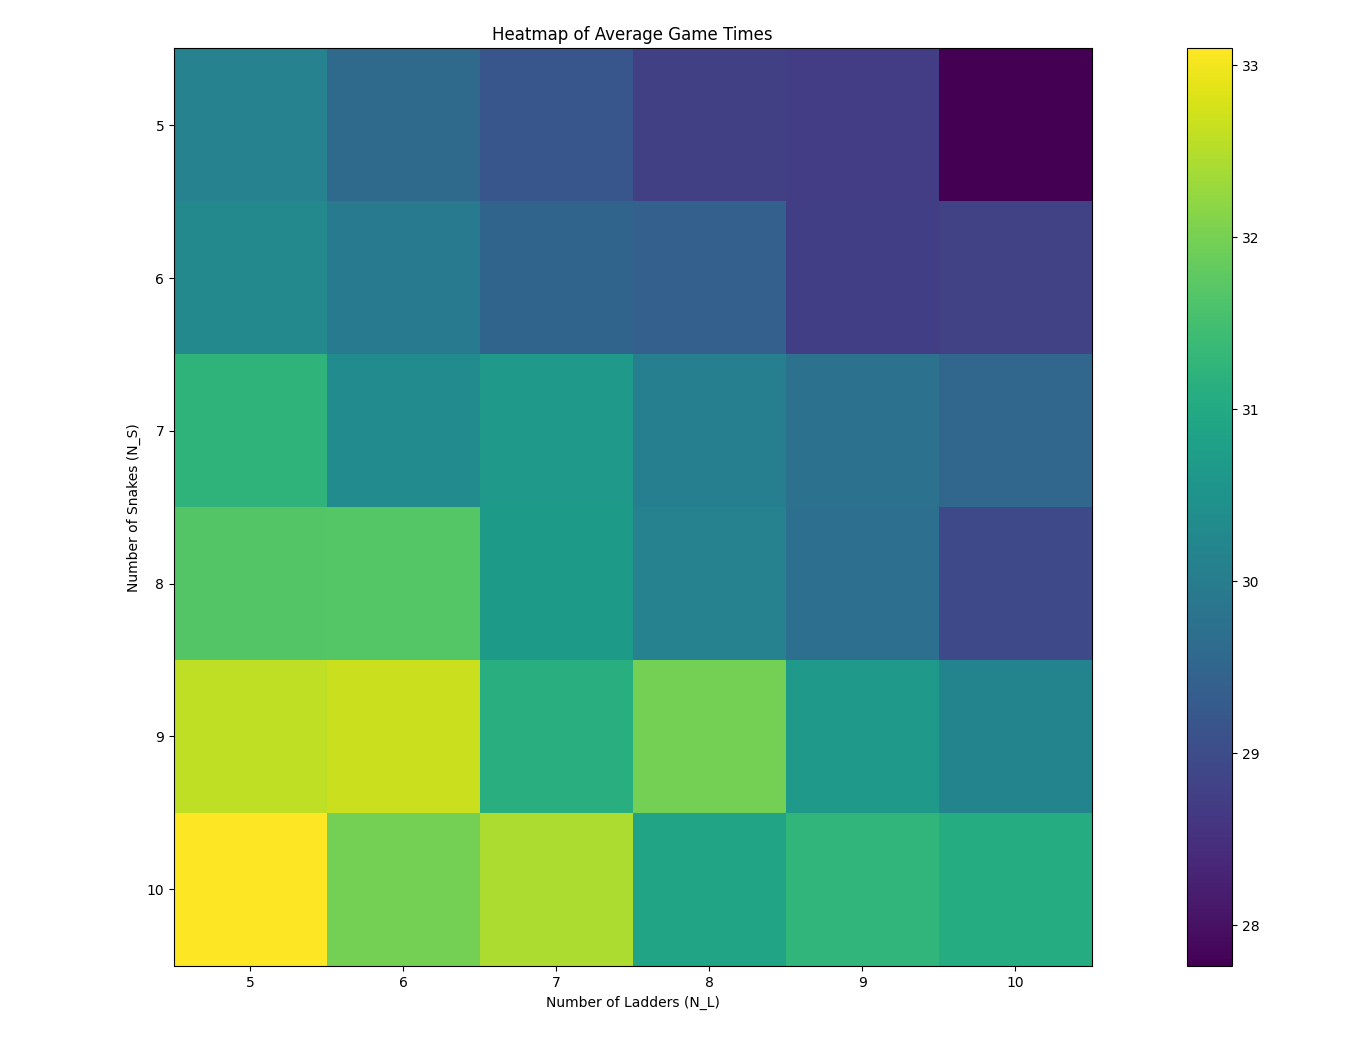
\includegraphics[width=0.8\linewidth]{Heatmap}
	\caption{Heatmap of Average Game Times}
	\label{fig:heatmap}
\end{figure}
	The heatmap (fig 1.3) visually overviews the interaction between $N_{S}$ and $N_{L}$ on average game time. Colours range from dark shades (indicating shorter game times) to bright shades (indicating longer game times). A clear pattern emerges from the heatmap, that suggests: as the number of ladders increases, the average game time decreases. This trend is most noticeable for higher snake counts ($N_{S} >= 9$), where additional ladders significantly reduce game times. The bottom-right corner of the heatmap ($N_{S} >= 9, N_{L} = 10$) shows the shortest game times, reinforcing the idea that ladders mitigate the delays caused by snakes. The effect of snakes on game time is not quite linear. For example, increasing the number of snakes from 5 to 6 does not dramatically change the game time. However, when the number of snakes is increased to 9 or 10, the game times rise substantially. This suggests a threshold beyond which additional snakes greatly increase the likelihood of players landing on them, thereby extending game time by a significant margin. This indicates that while snakes introduce challenges, their impact can be mitigated by providing players ample ladders to climb back up.
	
	\section{Conclusion}
	This study has been able to provide valuable quantitative insights into Snakes and Ladders, specifically focusing on how the number of snakes and ladders influences average game time. By simulating numerous games across various board configurations with fixed snake and ladder lengths, the project has been able to discern trends and patterns that contribute to a deeper understanding of this classic game and the parameters that influence how the game inherently feels. The findings presented reveal various insights such as, the number of snakes having a clear effect on the average game time as count of snakes increases, while the impact of number of ladders on the game makes it more consistent and sometimes decreasing the game time. The presence of outliers and fluctuating trend lines underscores the significant influence of board layout, where strategic placement of snakes and ladders can create ``traps'' or ``shortcuts'' (as a means to quickly progress or regress on the board), leading to substantial variations in game duration. This chapter serves as a foundation for further exploration into game mechanics of Snakes and Ladder but it also suggests that looking into other variables like the lengths could also provide much needed insight into their dynamics as game modifiers. As the project continues to explore the intricate interplay of chance and strategy in games like Snakes and Ladders, it seeks to pave the way for a more informed and nuanced approach to game design, enriching the landscape of interactive entertainment.	
\end{document}
